%%%%%%%%%%%%%%%%%%%%%%%%%%%%%%%%%%%%%%%%%%%%%%
%                insertmeeting
% 1) Title (something creative & funny?)
% 2) Date (MM/DD/YYYY)
% 3) Location (ex. Hagerty High School)
% 4) People/Committees Present 
% 5) Picture 
% 6) Start Time & Stop Time (ex. 12:30AM to 4:30PM)
%%%%%%%%%%%%%%%%%%%%%%%%%%%%%%%%%%%%%%%%%%%%%%
\insertmeeting 
	{Mecanum Madness} 
	{09/30/21}
	{Hagerty High School}
	{Clayton, Jensen, Nathan, Ritam}
	{Images/RobotPics/robot.jpg}
	{2:30 - 4:30}
	
\hhscommittee{Hardware}
\noindent\hfil\rule{\textwidth}{.4pt}\hfil
\subsubsection*{Goals}
\begin{itemize}
    \item Set up field
    \item Test mecanum drive
 

\end{itemize} 

\noindent\hfil\rule{\textwidth}{.4pt}\hfil

\subsubsection*{Accomplishments}
After getting the mecanum drivetrain rebuilt last meeting, we are almost ready to test. Before we can, however, we need to set up the field. Because our school also has two vex teams, we have to share the field, so we started setting up half of the field for Freight Frenzy. Although we have already set up the carousel, we still needed to add all of the tape and the barriers (image 1). While setting up the barriers, we realized that if they weren’t ziptied really tight, they shifted slightly. This might make it harder for the robot to go over  them during a competition if they aren’t set up really well. Noticing this, we noted that we will need to ensure our robot can still get over the barriers even if they are a bit loose. Once the barriers were up, we reorganized the wires on the drivetrain to prevent them from getting caught in the wheels or interfering with our testing in any way (image 2). 
Finally, it was time to test the mecanum drive. Just as we had hoped, the mecanum drivetrain flew over the  barriers with little issue. Because of the shape of the drivetrain (image 4), the wheels hit the pipes before the drive plates do, making it easily pull itself over the barrier. On the back of the drivetrain, we didn’t design a cutout for the wheels, making the plates and the wheels hit the  pipes at about the same time. We noticed that although the robot could still drive over the barriers backwards, it isn’t nearly as smooth. This clearly necessitates the need for a wheel cutout on both sides. Seeing how the mecanum drive performed, we are optimistic about the tank drive, which will have more traction than the mecanum drive does. With the addition of the middle drop center wheel, the possibility of getting stuck should be reduced. That being said, the tank drive design that we currently have to test has much lower plates and motors, so in its current state, it may not go over the barrier as smoothly. We were already planning on making some design changes, but we still hope to test the current design soon.

 

\begin{figure}[ht]
\centering
\begin{minipage}[b]{.48\textwidth}
  \centering
  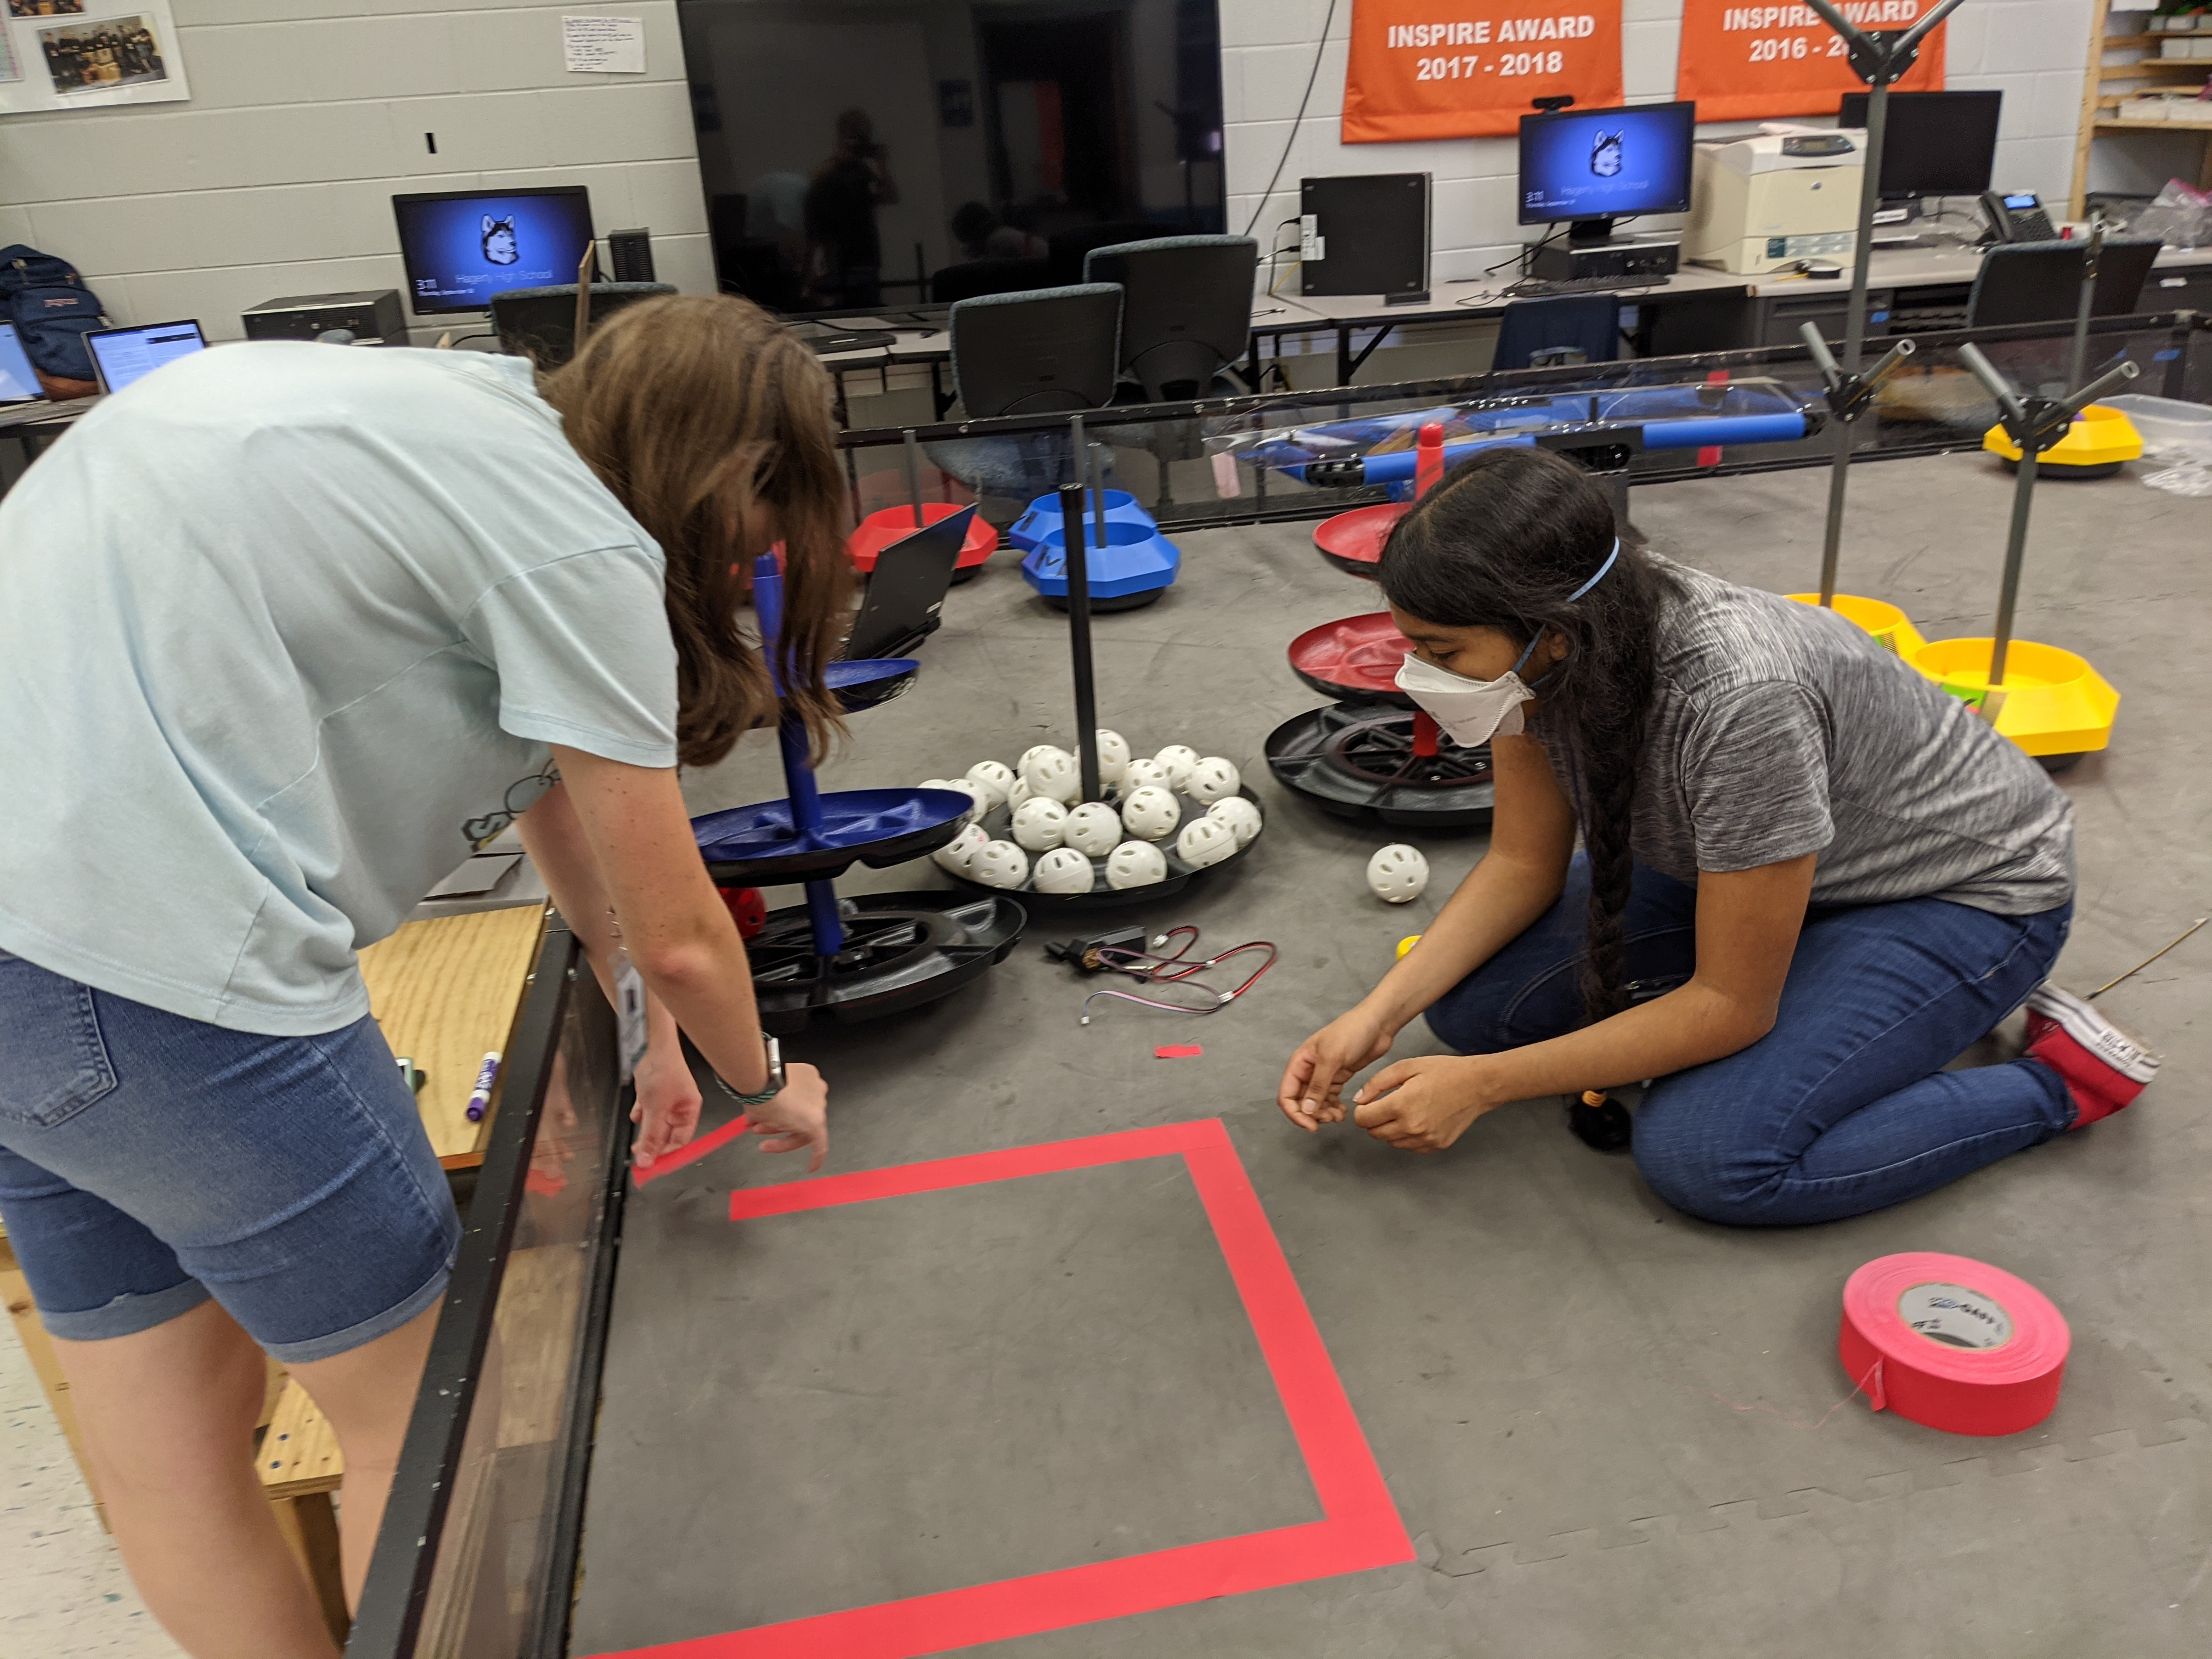
\includegraphics[width=0.95\textwidth]{Meetings/September/09-30-21/9-30-21_Hardware_Image1 - Nathan Forrer.jpg}
  \caption{Anouska and Samantha setting up the field with tape.}
  \label{fig:pic1}
\end{minipage}%
\hfill%
\begin{minipage}[b]{.48\textwidth}
  \centering
  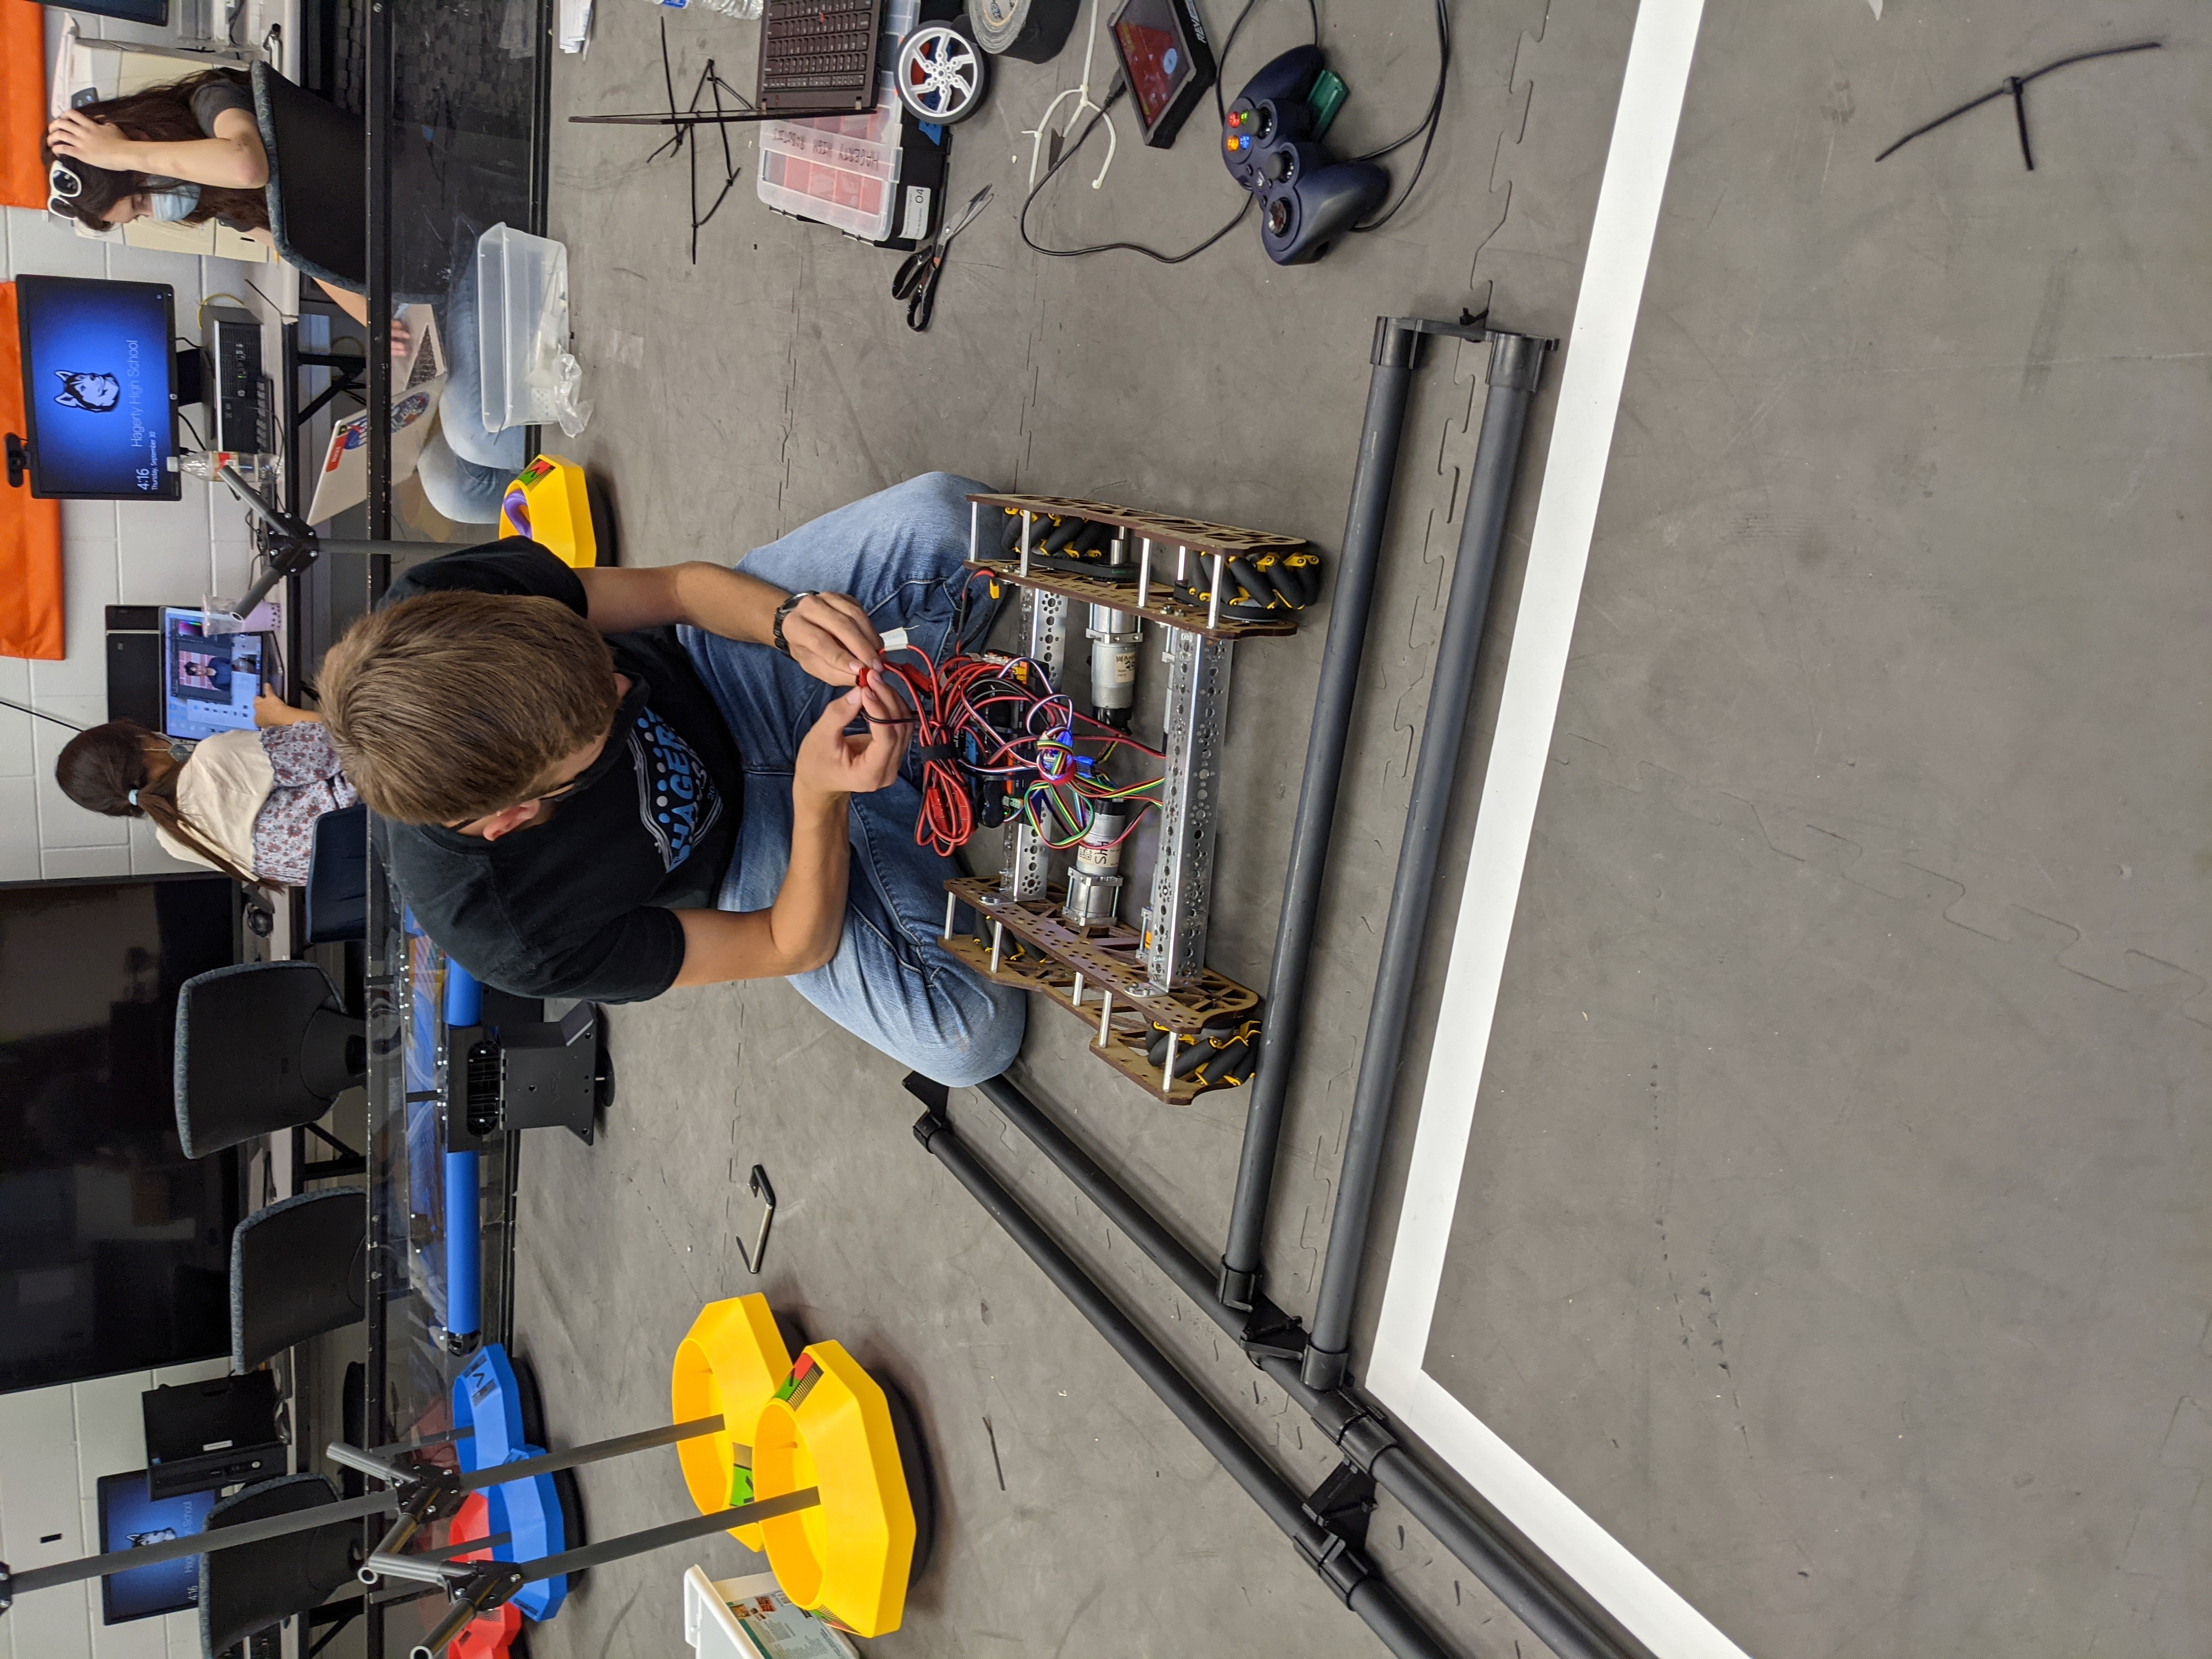
\includegraphics[width=0.95\textwidth]{Meetings/September/09-30-21/9-30-21_Hardware_Image2 - Nathan Forrer.jpg}
  \caption{Jensen wiring the Mecanum drive.}
  \label{fig:pic2}
\end{minipage}
\end{figure}

\begin{figure}[ht]
\centering
\begin{minipage}[b]{.48\textwidth}
  \centering
  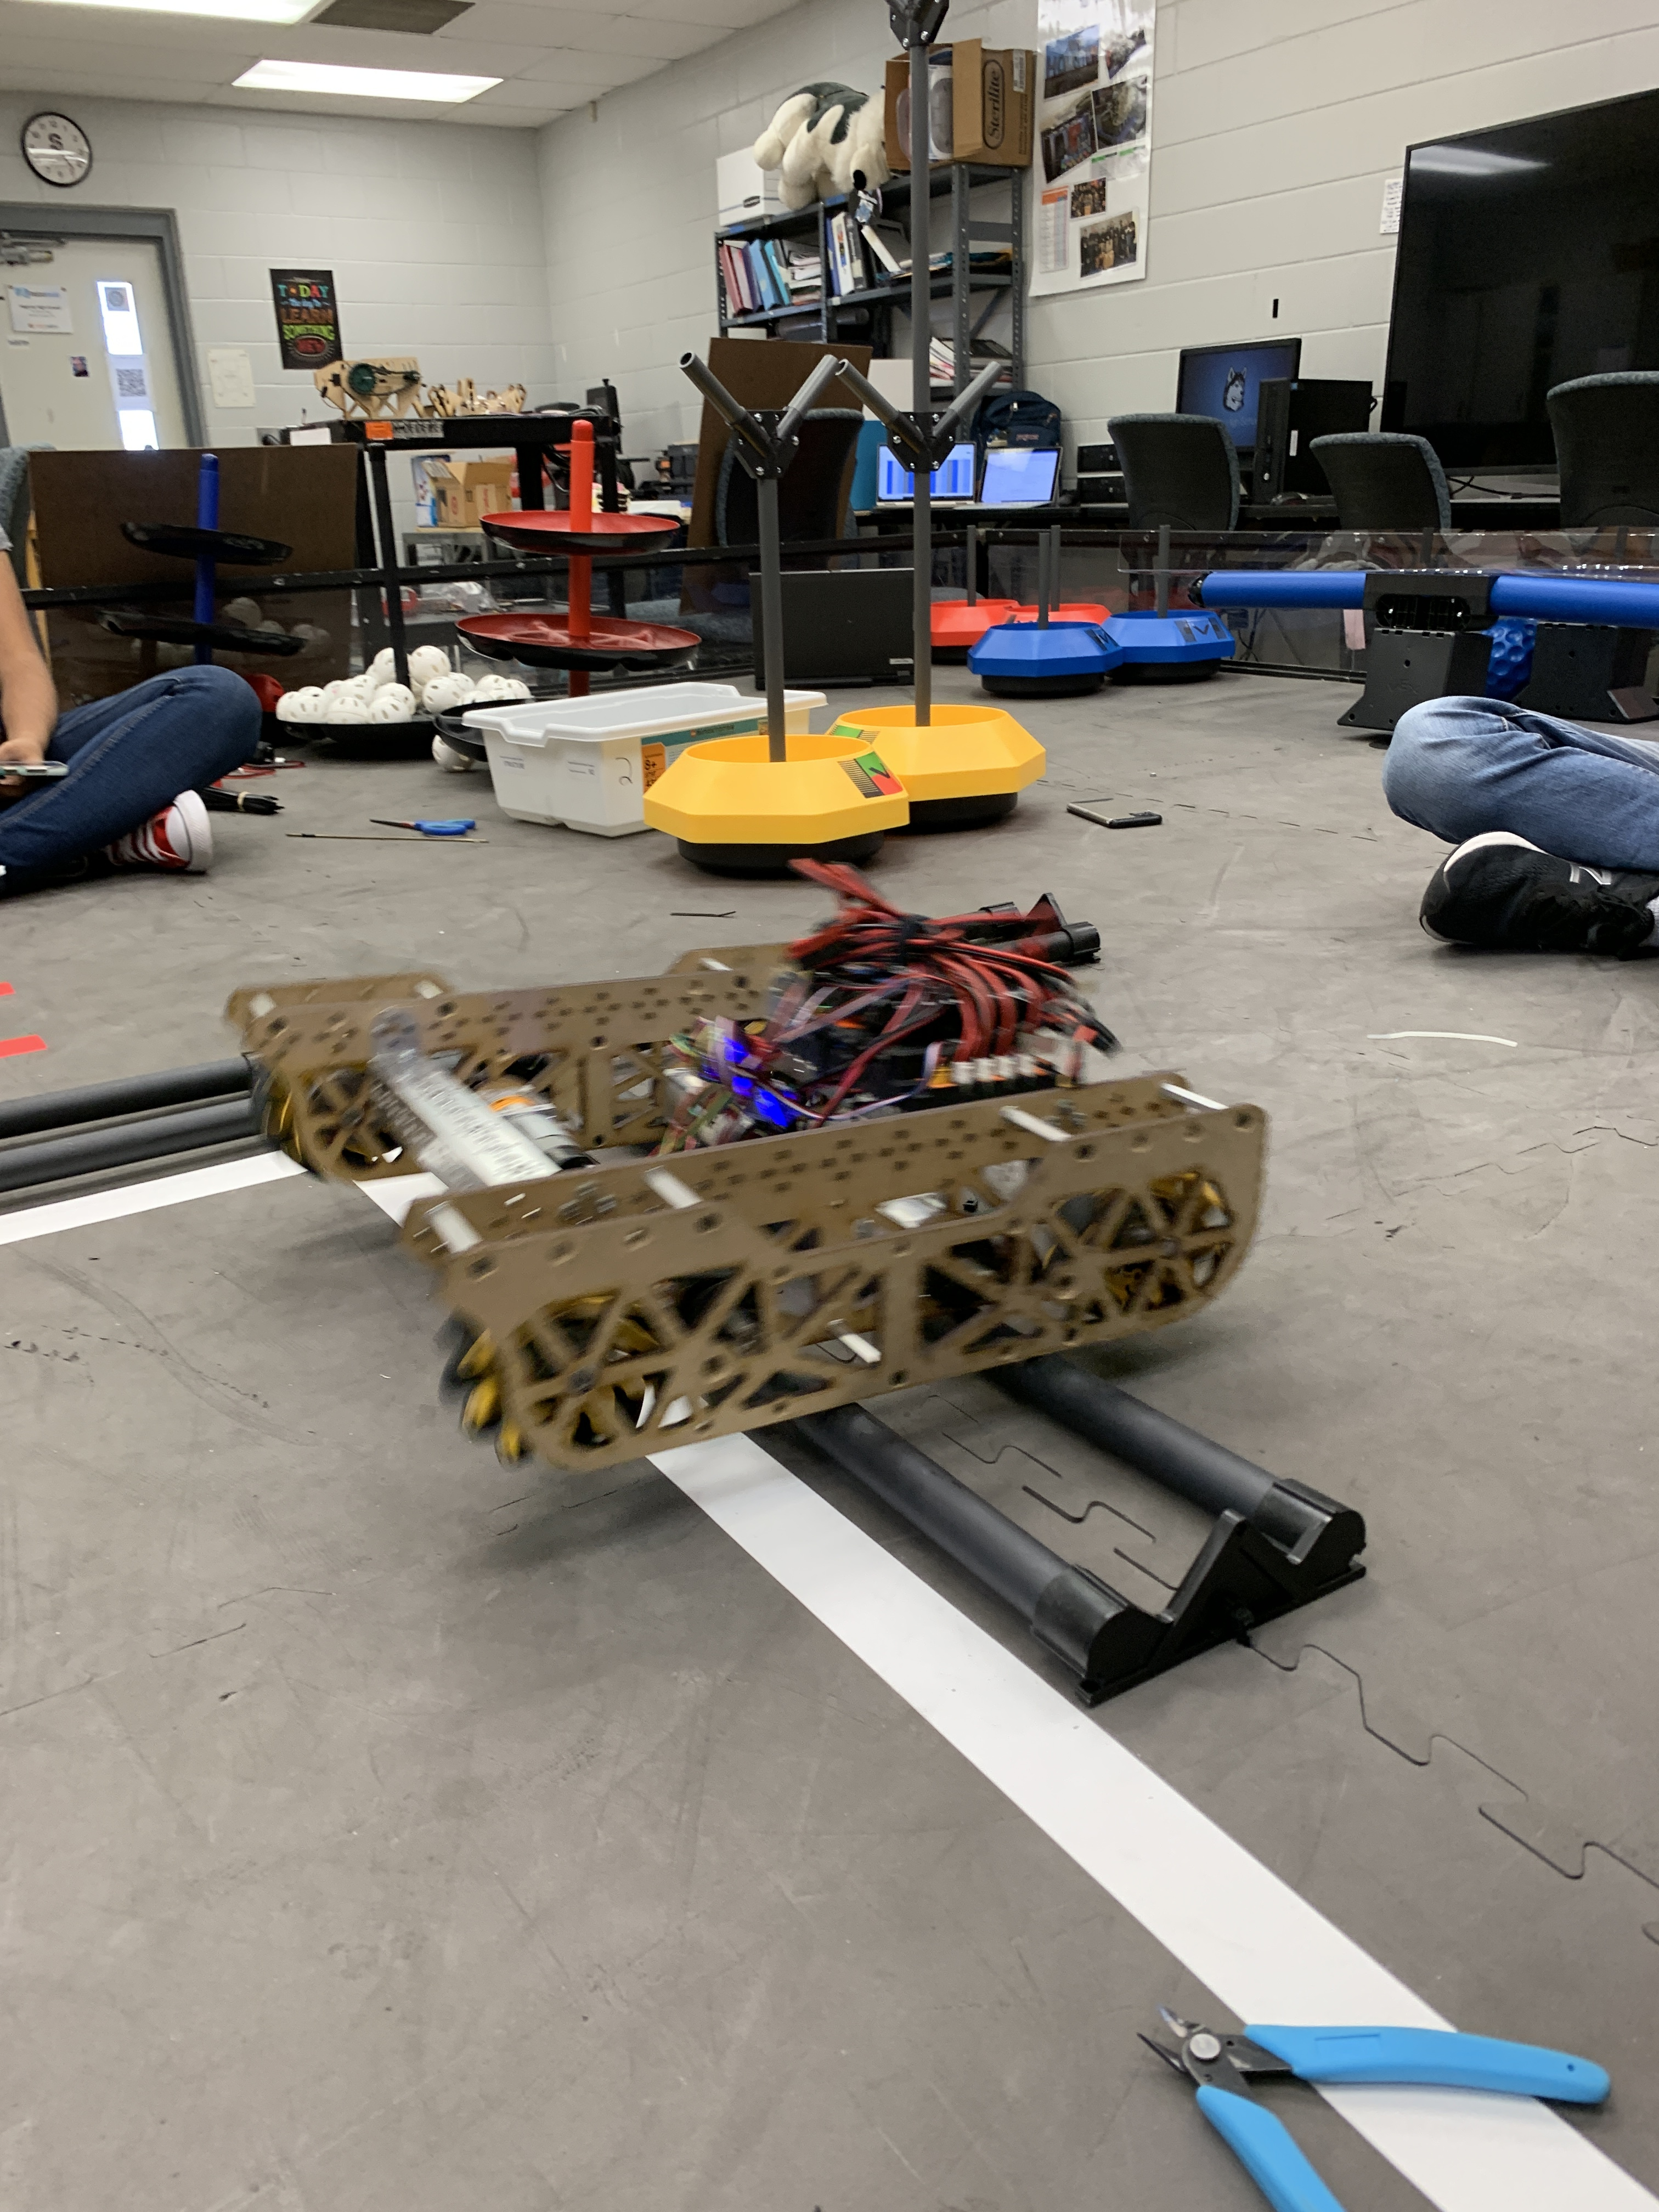
\includegraphics[width=0.95\textwidth]{Meetings/September/09-30-21/9-30-21_Hardware_Image3 - Nathan Forrer.JPG}
  \caption{Testing the mecanum drive's ability to move over the barrier.}
  \label{fig:pic1}
\end{minipage}%
\hfill%
\begin{minipage}[b]{.48\textwidth}
  \centering
  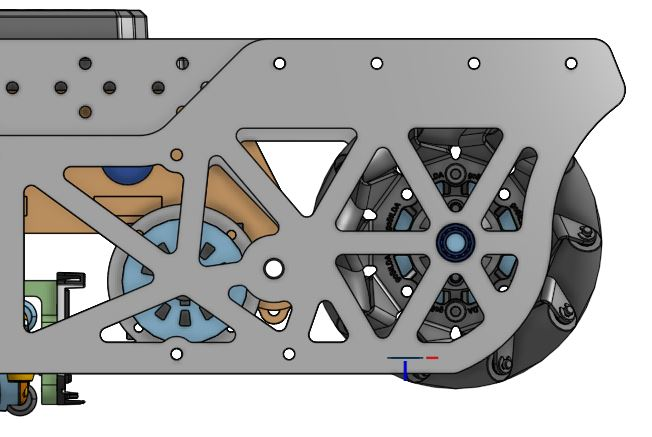
\includegraphics[width=0.95\textwidth]{Meetings/September/09-30-21/9-30-21_Hardware_Image4 - Nathan Forrer.JPG}
  \caption{Our CAD drawing for the driveplates.}
  \label{fig:pic2}
\end{minipage}
\end{figure}

\whatsnext{
\begin{itemize}
    \item Test tank drive
    \item Build prototype 4 wheel tank drive

\end{itemize} 
}